\section{课程名称}

分布式系统。

\section{实验项目名称}

SDCS: Simple Distributed Cache System.

\section{实验原理}

RPC是一种远程过程调用协议,它是一种通过网络从远程计算机程序上请求服务,而不需要了解底层网络技术的协议。一个完整的RPC架构里面包含了四个核心的组件,分别是客户端、客户端存根、服务端、服务端存根。

\begin{figure}[H]
    \centering
    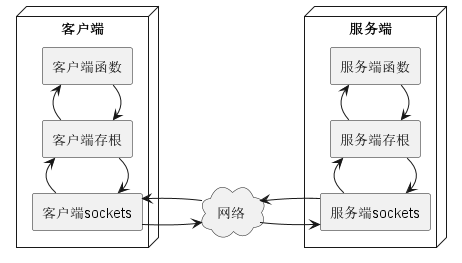
\includegraphics[width=\textwidth]{examples/rpc原理.png}
    \caption{RPC原理}
    \label{fig:rpc}
\end{figure}

如图\ref{fig:rpc}所示,当客户端请求RPC服务时,会通过存根打包请求参数,然后通过网络发送给服务端;服务端存根接收请求,将消息解包后调用本地方法,并将结果返回到客户端。为了使得请求可以在网络中传递,往往需要对数据进行序列化操作。

\section{实验目的}

完成一个简易分布式缓存系统,并实现如下功能:
\begin{itemize}
    \item 键值对的保存和读取。用户可将数据组织成键值对形式保存到数据库中,并通过指定的键读取数据。键的类型是字符串,而值可以是任意类型。
    \item 节点通信。各个节点之间通过RPC通信完成信息交换。
    \item 基本的负载均衡。数据将会根据键的内容被均匀分布给各个节点,读取时也会根据键的内容到指定的节点中获取值。
    \item 快速部署。本系统通过docker和docker-compose进行集成,用户可通过一行命令启动或停止分布式服务。如果要增删节点,用户只需编辑docker-compose中的内容。
\end{itemize}

\section{实验内容}

完成一个简易分布式缓存系统,其具体要求如下。

\begin{enumerate}
    \item Cache数据以Key-value形式存储在缓存系统节点内存中(不需要持久化)。
    \item Cache数据以既定策略(round-robin或hash均可,不做限定)分布在不同节点(不考虑副本存储)。
    \item 服务至少启动3个节点,不考虑节点动态变化:
    \begin{enumerate}
        \item 所有节点均提供HTTP访问入口。
        \item 客户端读写访问可从任意节点接入,每个请求只支持一个key存取。
        \item 若数据所在存储服务器与接入服务器不同,接入服务器通过内部RPC从目标存储服务器获取数据,再返回至客户端。
    \end{enumerate}
\end{enumerate}